%AUTOR: KAMIL ŁANGOWSKI 
%EMAIL: kamil.langowski@gmail.com
\documentclass[a4paper]{article}

\usepackage{polski}
\usepackage{amsfonts}
\usepackage{listings}
\usepackage{graphicx}
\usepackage{tikz}
\usepackage{geometry}
\usepackage{hyperref}


\lstdefinestyle{mystyle}{
    basicstyle=\ttfamily\footnotesize,
    breakatwhitespace=false,         
    breaklines=true,                 
    captionpos=b,                    
    keepspaces=true,                 
    numbers=left,                    
    numbersep=5pt,                  
    showspaces=false,                
    showstringspaces=false,
    showtabs=false,                  
    tabsize=2
}

\lstset{style=mystyle}
\newtheorem{defi} {Definicja}
\newtheorem{twi}{Twierdzenie}

\title{Maszyna wektorów nośnych}
\author{Kamil Łangowski \\ Wydział Fizyki Technicznej i Matematyki Stosowanej \\ Politechnika Gdańska}
\begin{document}
\maketitle
\newpage
\section{Teoria}
Maszyna wektorów nośnych (ang.  \textit{support vector machine}, SVM) to model nadzorowanego uczenia maszynowego, który znajduje zastosowanie w zadaniach związanych zarówno z klasyfikacją, jak i regresją. Omawiając SVM w głównej mierze skupimy się na zastosowaniach w problemach klasyfikacji. Zanim jednak zajmiemy się maszyną wektorów nośnych, w celu zapobiegnięcia niedomówień, musimy wprowadzić model zwany klasyfikatorem maksymalnego marginesu (ang. \textit{maximal margin classifier}). Następnie uogólnimy go otrzymując klasyfikator wektorów nośnych (ang. support \textit{vector classifier}), który z kolei uogólnia się do maszyny wektorów nośnych. Często można spotkać się z sytuacją, w której to każdy z przytoczonych powyżej modeli występuje pod nazwą "maszyna wektorów nośnych".

\subsection{Klasyfikator maksymalnego marginesu}
Konstruując klasyfikator maksymalnego marginesu bazować będziemy na pojęciu hiperpłaszczyzny, tzn. $d-1$ wymiarowej podprzestrzeni afinicznej pewnej przestrzeni $d$-wymiarowej (np. hiperpłaszczyzna w przestrzeni 2-wymiarowej jest krzywą).
\begin{defi}[Hiperpłaszczyzna]
Hiperpłaszczyzna w przestrzeni $d$-wymiarowej  dla obserwacji \\$x = (x^{(1)},x^{(2)},\dots,x^{(d)})$ opisana jest przez równanie 
\begin{equation}\label{(2.38)}
    \beta_0 + \sum\limits_{i=1}^d{\beta_ix^{(i)}} = 0,
\end{equation}
gdzie $\beta_0, \beta_1, \dots, \beta_d$ są parametrami równania.
\end{defi}
Jeżeli pewna obserwacja $x=(x^{(1)}, x^{(2)}, \dots, x^{(d)})$ spełnia równanie (1), wówczas punkt ten znajduje się na rozważanej hiperpłaszczyźnie. Natomiast, jeżeli $x$ nie spełnia (1) oraz zachodzi 
\begin{equation}
    \beta_0 + \sum\limits_{i=1}^d{\beta_ix^{(i)}} < 0,
\end{equation}
oznacza to, że $x$ znajduje się po jednej ze stron hiperpłaszczyzny. W analogiczny sposób określone jest położenie punktu $x$, po drugiej ze stron. Mianowicie 
\begin{equation}
\beta_0 + \sum\limits_{i=1}^d{\beta_ix^{(i)}} > 0.
\end{equation}
Widzimy zatem, że hiperpłaszczyzna rozdziela $d$-wymiarową przestrzeń na dwie odrębne  części. Ponadto posiadając informacje na temat parametrów hiperpłaszczyzny, bez trudu możemy zdeterminować, po której ze stron znajduje się rozważany punkt.
\begin{figure}[ht]
    \centering
    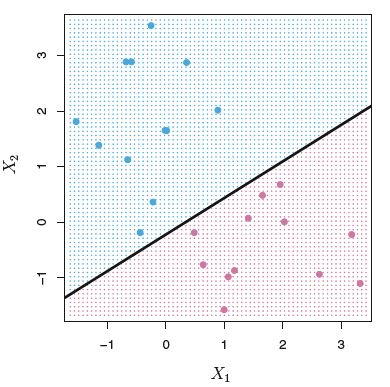
\includegraphics[width = 180 pt, height = 140 pt]{SVM!.JPG}
    \caption{Hiperpłaszczyzna rozdzielająca dwie klasy obserwacji. Na powyższym rysunku $X_1 =\\= X^{(1)}$ oraz $X_2 = X^{(2)}$.}
\end{figure}
\newpage
Załóżmy, że $X$ jest $n\times d$ wymiarową macierzą zawierającą $n$-wymiarowe obserwacje 
\begin{equation}
    x_1 = \left( \begin{array}{c}
    x_{1}^{(1)}  \\
    x_{1}^{(2)} \\
    \vdots \\
    x_{1}^{(d)} 
    \
\end{array} \right)^T, 
\dots,x_n = \left( \begin{array}{c}
    x_{n}^{(1)}  \\
    x_{n}^{(2)} \\
    \vdots \\
    x_{n}^{(d)} 
    \
\end{array} \right)^T.
\end{equation}
Ponadto niech każda z rozważanych obserwacji należy do jednej z dwóch klas $y\in\{-1,1\}=Y$. Załóżmy także, że mamy pewną obserwację testową $x_j = (x_j^{(1)},x_j^{(2)},\dots , x_j^{(d)})$. Podobnie jak w przypadku regresji logistycznej chcemy uzyskać klasyfikator, za pomocą którego będziemy mogli określić przynależność rozważanej obserwacji testowej. W tym celu posłużymy się pojęciem hiperpłaszczyzny separującej (ang. \textit{separating hyperplane}).
\begin{defi}[Hiperpłaszczyzna separująca]
Hiperpłaszczyzna separująca to hiperpłaszczyzna, która jednoznacznie rozdziela obserwacje należące do różnych klas.
\end{defi}
Oznacza to, że obserwacje należące do klasy 1 znajdują się po jednej stronie hiperpłaszczyzny separującej, a obserwacje należące do klasy $-1$ po przeciwnej. Przykładowo 
\begin{equation}\label{(2.42)}
\left\{ \begin{array}{ll}
\beta_0 + \sum\limits_{i=1}^d{\beta_ix_{j}^{(i)}} > 0 ,\quad\textrm{gdy $y_j = 1$}  \\
\beta_0 + \sum\limits_{i=1}^d{\beta_ix_{j}^{(i)}} < 0 ,\quad\textrm{gdy $y_j = -1$}  
\end{array} \right.
\end{equation}
\indent Zatem, w przypadku istnienia hiperpłaszczyzny separującej, możemy z niej skorzystać w celu konstrukcji klasyfikatora binarnego. Niech $f(x_j) = \beta_0 + \sum_{i=1}^d{\beta_ix_{j}^{(i)}}$. w przypadku, gdy $f(x_j) > 0$ obserwacja $x_j$ należy do klasy 1, natomiast dla $f(x_j) < 0$ obserwacja $x_j$ należy do klasy $-1$. Zauważmy także, że jeśli $f(x_j)$ osiąga wartości bliskie zeru, to obserwacja $x_j$ znajduje się bliżej hiperpłaszczyzny, analogicznie dla dalszych obserwacji.
Przewidywaną klasę obserwacji testowej $x_j$ możemy zapisać także jako 
\begin{equation}
    y_j = \textrm{sign}\left(f(x_j\right),
\end{equation}
gdzie $\textrm{sign}$ jest funkcją znaku.
\\\indent Jeśli dane jakim się zajmujemy mogą być doskonale rozdzielone poprzez hiperpłaszczyznę, wtedy istnieje nieskończona liczba hiperpłaszczyzn separujących. Z tego względu należy wybrać hiperpłaszczyznę, która w najlepszy sposób będzie spełniała rolę klasyfikatora. Sposobem na wybór takiej hiperpłaszczyzny separującej jest hiperpłaszczyzna maksymalnego marginesu (ang. \textit{maximal margin hyperplane}), która wyróżnia się tym, iż jest najbardziej oddalona od wszystkich obserwacji. Mając zadaną hiperpłaszczyznę rozdzielającą, wyznaczamy odległość punktów obserwacji od niej oraz wybieramy tę, która jest najmniejsza -- nazywamy ją marginesem. Hiperpłaszczyzna maksymalnego marginesu to hiperpłaszczyzna, dla której margines jest największy. Za pomocą takiej hiperpłaszczyznę możemy klasyfikować obserwacje na podstawie ich położenia względem niej. Tak powstały klasyfikator nazywany jest klasyfikatorem maksymalnego marginesu. W takim podejściu do klasyfikacji zakładamy, że duży margines dla danych treningowych będzie także odpowiedni dla danych testowych. \\\indent  W praktyce klasyfikator maksymalnego marginesu często działa poprawnie, jednak w przypadku obserwacji o dużym wymiarze ma skłonności do nadmiernego dopasowania. Na rysunku \ref{2.10} przedstawiono przykładową hiperpłaszczyznę maksymalnego marginesu. Odległość od ciemnej linii -- hiperpłaszczyzny separującej, do linii przerywanych jest marginesem hiperpłaszczyzny separującej. Zwróćmy uwagę, że trzy spośród najbliższych obserwacji do hiperpłaszczyzny maksymalnego marginesu są od niego równo oddalone. Te punkty nazywamy wektorami nośnymi (ang. \textit{support vectors}), ze względu na fakt, iż przesunięcie jakiegokolwiek z nich skutkowałoby przesunięciem hiperpłaszczyzny separującej. Problem konstrukcji klasyfikatora maksymalnego marginesu sprowadza się do odpowiedniego wyboru parametrów równania hiperpłaszczyzny separującej w taki sposób, by margines utworzony za pomocą wektorów nośnych był największy.
\begin{figure}[ht]
    \centering
    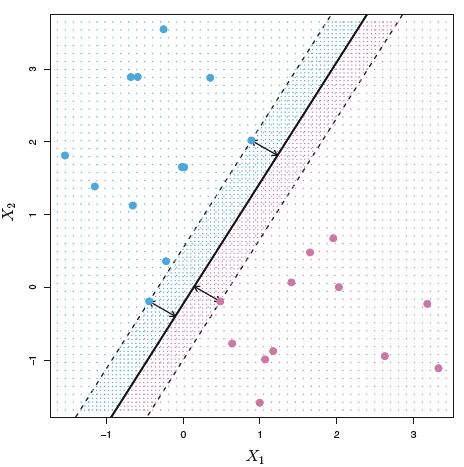
\includegraphics[width = 210 pt, height = 190 pt]{MAXMARGIN.JPG}
    \caption{Hiperpłaszczyzna maksymalnego marginesu. Na powyższym rysunku $X_1 = X^{(1)}$ oraz $X_2 = X^{(2)}$.}
    \label{2.10}
\end{figure}\newpage
\subsection{Klasyfikator wektorów nośnych}
Jeżeli niemożliwym jest rozdzielenie obserwacji hiperpłaszczyzną to posługujemy się klasyfikatorem wektorów nośnych. W odróżnieniu od klasyfikatora maksymalnego marginesu, klasyfikator wektorów nośnych nie wyznacza największego marginesu dla hiperpłaszczyzny separującej w sposób, by żadna z obserwacji nie znalazła się po stronie, do której nie należy. Natomiast pozwala na położenie niektórych obserwacji po niepoprawnej stronie hiperpłaszczyzny separującej. Umożliwia to dużo bardziej wydajną pracę klasyfikatora w przypadkach, dla których klasyfikator maksymalnego marginesu nie miałby szans powodzenia. Klasyfikacja dokonywana jest na podobnych zasadach co w (5). Jednakże w problemie optymalizacji klasyfikatora występują pewne parametry (\textit{slack parameters}), które pozwalają niewielkiej liczbie przypadków na niepoprawną klasyfikację. 
\subsection{Maszyna wektorów nośnych}
Maszyna wektorów nośnych jest rozszerzeniem koncepcji klasyfikatora wektorów nośnych poprzez zwiększenie przestrzeni cech z wykorzystaniem jąder (ang. \textit{kernels}). Zagadnienia związane z SVM oraz z jądrami nie są trywialne zatem w tej sekcji przedstawimy ten problem tylko pobieżnie. SVM jest podejściem do klasyfikacji, w którym granica decyzyjna (hiperpłaszczyzna separująca) nie musi być liniowa.  W przypadku, gdy liniowa granica decyzyjna nie spełnia swojego zadania, możliwe jest powiększenie przestrzeni cech o obserwacje podniesione np. do drugiej potęgi. W ten sposób rozwiązuje się problem nieliniowości. To rozwiązanie niesie jednak ze sobą niebezpieczeństwo powstania liczby danych, z którą komputerowi będzie bardzo trudno sobie poradzić. SVM pozwala na powiększenie przestrzeni cech w sposób najbardziej wydajny. Dokonuje tego za pomocą funkcji nazywanej jądrem, która jest miarą podobieństwa dwóch obserwacji (uogólnienie iloczynu skalarnego). Można powiedzieć także, że jądro to funkcja określająca w sposób ilościowy podobieństwo dwóch obserwacji. Przykładowy wzór
\begin{equation}\label{(2.44)}
    K(x_j, x_{j'}) = \sum\limits^d_{i=1}x_{j}^{(i)}x_{j'}^{(i)},
\end{equation} 
gdzie $K$ jest jądrem, a $x_j$ i $x_{j'}$ są badanymi obserwacjami. Jądro  postaci (2.44) w rezultacie zastosowania do SVM daje nam klasyfikator wektorów nośnych. Jeśli jądro jest funkcją nieliniową mówimy o SVM. 
\newpage
\section{Przykład}
\subsection{Opis zbioru}
W przykładzie implementacji SVM posłużymy się zbiorem danych z pakietu \textit{MASS} o nazwie \textit{cats}. Zbiór zawiera informacje na temat masy serca i masy ciała kotów obu płci. Wszystkie badane koty były osobnikami dorosłymi i ważyły co najmniej 2 kg. 
\subsection{Cel}
Naszym celem będzie zastosowanie maszyny wektorów nośnych do zaklasyfikowania płci danego kota na podstawie masy ciała i masy serca.
\subsection{Kod programu}
W pierwszym kroku ładujemy pakiety, z których będziemy korzystali
\begin{lstlisting}[language=R, frame=single]
library(MASS)
library(e1071)
library(caret)
library(OneR)
library(BBmisc)
\end{lstlisting}
Pakiet \textit{Mass}, tak jak wspomnieliśmy, zawiera zbiór \textit{cats}. Sprawdzamy więcej informacji na temat naszego zbioru danych:
\begin{lstlisting}[language=R, frame=single]
data(cats)
dane <- cats

str(dane)
summary(dane)
\end{lstlisting}
\begin{lstlisting}[language=R, frame=single]
'data.frame':	144 obs. of  3 variables:
 $ Sex: Factor w/ 2 levels "F","M": 1 1 1 1 1 1 1 1 1 1 ...
 $ Bwt: num  2 2 2 2.1 2.1 2.1 2.1 2.1 2.1 2.1 ...
 $ Hwt: num  7 7.4 9.5 7.2 7.3 7.6 8.1 8.2 8.3 8.5 ...
 
  Sex         Bwt             Hwt       
 F:47   Min.   :2.000   Min.   : 6.30  
 M:97   1st Qu.:2.300   1st Qu.: 8.95  
        Median :2.700   Median :10.10  
        Mean   :2.724   Mean   :10.63  
        3rd Qu.:3.025   3rd Qu.:12.12  
        Max.   :3.900   Max.   :20.50
\end{lstlisting}
Zbiór zawiera 144 obserwacje o trzech cechach, kolejno:
\begin{itemize}
    \item \textit{Sex} -- płeć danego kota (kategoryczna zmienna celu),
    \item \textit{Bwt} -- masa jego ciała (zmienna numeryczna),
    \item \textit{Hwt} -- masa jego serca (zmienna numeryczna). 
\end{itemize} W rozważanym zbiorze liczba samców to 97, a samic 47. Tworzymy model SVM dla całego zbioru w celu wizualizacji:
\begin{lstlisting}[language=R, frame=single]
model_dane <- svm(Sex ~ ., data = dane)
print(model_dane)
\end{lstlisting}

\begin{figure}[ht]
    \centering
    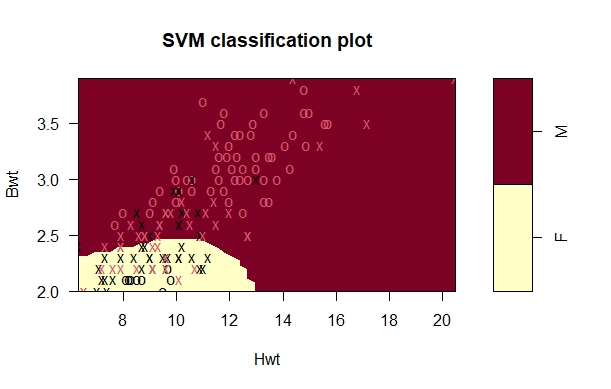
\includegraphics[width = \textwidth]{SVM.jpeg}
    \caption{Zastosowanie maszyny wektorów nośnych do zbioru \textit{cats}.}
    \label{r(2.11)}
\end{figure}
Na rysunku \ref{r(2.11)} przedstawiona jest granica decyzyjna dla naszego przypadku. Żółta część oznacza strefę klasyfikacji nowej obserwacji jako osobnika płci żeńskiej, z kolei część czerwona jako osobnika płci męskiej.\newpage
Za pomocą funkcji \textit{normalize} normalizujemy dane:
\begin{lstlisting}[language=R, frame=single]
dane_norm <- normalize(dane, method = "range", range = c(0,1))
\end{lstlisting}
W celu kontroli wyświetlamy 6 początkowych i 6 końcowych wierszy oraz podsumowanie informacji o znormalizowanych danych
\begin{lstlisting}[language=R, frame=single]
head(dane_norm)
tail(dane_norm)
\end{lstlisting}
\begin{lstlisting}[language=R, frame=single]
  Sex        Bwt        Hwt
1   F 0.00000000 0.04929577
2   F 0.00000000 0.07746479
3   F 0.00000000 0.22535211
4   F 0.05263158 0.06338028
5   F 0.05263158 0.07042254
6   F 0.05263158 0.09154930

    Sex       Bwt       Hwt
139   M 0.8421053 0.6126761
140   M 0.8947368 0.3309859
141   M 0.9473684 0.5985915
142   M 0.9473684 0.7394366
143   M 1.0000000 0.5704225
144   M 1.0000000 1.0000000
\end{lstlisting}
Zwróćmy uwagę, że pojawiły się wartości zerowe. Nie jest to niewłaściwe dlatego, że wartości najmniejsze tzn. wagę 2 kg zastąpiono wartością 0.
\newpage
Dokonujemy podziału zbioru na zbiór treningowy i zbiór testowy w stosunku 3:2, a następnie tworzymy model maszyny wektorów nośnych:
\begin{lstlisting}[language=R, frame=single]
podzial <- createDataPartition(dane_norm$Sex, p = 0.60, list = FALSE)
trening <- dane[podzial, ] 
test <- dane[-podzial, ]
model_trening <- svm(Sex ~ ., data = trening)
\end{lstlisting}
Wykonujemy predykcję i wyświetlamy informacje na temat modelu:
\begin{lstlisting}[language=R, frame=single]
predykcja <- predict(model_trening, test[, -1], type = "class")
eval_model(predykcja, test[,1])
\end{lstlisting}
\begin{lstlisting}[language=R, frame=single]
Confusion matrix (absolute):
          Actual
Prediction  F  M Sum
       F    8  6  14
       M   10 32  42
       Sum 18 38  56

Confusion matrix (relative):
          Actual
Prediction    F    M  Sum
       F   0.14 0.11 0.25
       M   0.18 0.57 0.75
       Sum 0.32 0.68 1.00

Accuracy:
0.7143 (40/56)

Error rate:
0.2857 (16/56)

Error rate reduction (vs. base rate):
0.1111 (p-value = 0.3392)
\end{lstlisting}
Nasz model dokonał poprawnej predykcji płci kota 40 razy na 56 badane przypadki, co daje dokładność na poziomie $71.43\%$. 6 osobników płci męskiej zaklasyfikowano jako osobniki płci żeńskiej i 10 osobników płci żeńskiej zaklasyfikowano jako osobniki płci męskiej.
\end{document}